\documentclass[a4paper, 10pt]{article}
\usepackage[margin = 1in]{geometry}
\usepackage{amsmath}
\usepackage{tabularx}
\usepackage{framed}
\setlength{\parindent}{0em}
\newcolumntype{L}{>{\arraybackslash}m{10cm}}
\newcolumntype{T}{>{\arraybackslash}m{6cm}}
\usepackage{graphicx}
\usepackage{pdfpages}

\begin{document}

\section*{Topic 10 - Oscillations}
\section{Simple Harmonic Motion}
\begin{framed}
   \textbf{Simple harmonic motion} is defined as the motion of a particle about a fixed point such that its acceleration is proportional to its displacement from the fixed point and is always directed towards the fixed point

   \[
   a \propto -x
   \]
   \[
   a = -\omega^2 x
   \]
   where $\omega$ is the angular frequency of oscillation
\end{framed}	
\begin{itemize}
   \item Magnitude of acceleration is the largest at maximum displacement, and zero at equilibrium position
   \item Magnitude of velocity is the largest at equilibrium position, and zero at maximum displacement
\end{itemize}	

\textbf{Angular frequency}: is defined as the rate of change of phase angle of oscillation, and is equal to the product of $2\pi$ and its frequency
   \[
   \omega = 2\pi f
   \]

\textbf{Amplitude}: is the magnitude of the maximum displacement of the particle from its equilibrium position 
\textbf{Period, T}: the tie taken for one complete oscillation
\textbf{Frequency, F}: the number of oscillations per unit time
\[
 T = \frac{2\pi}{\omega},\ \omega = \frac{2\pi}{T}
\]

\subsection{Equations for S.H.M.}
For the case where particle is at maximum positive displacement initially, i.e. $x = x_0$ when $t = 0$:

displacement: 
\[
x = x_0 cos \omega t
\]

velocity: 
\[
v = -x_0 \omega sin \omega t
\]

aceeleration:
\[
a = -x_0 \omega^2 cos \omega t
\]

additionally,
\begin{align*}
   v &= -x_0 \omega sin \omega t \\
     &= -x_0 \omega \left( \pm  \sqrt{1 - cos^2 \omega t} \right) \\
     &= \pm \omega \sqrt{x_0^2 (1 - cos^2 \omega t} \\
     &= \pm \omega \sqrt{x_0^2 - x_0^2 cos^2 \omega t} \\
\end{align*}	

\[
   v = \pm \omega \sqrt{x_0^2 - x^2}
\]

and
\begin{align*}
   a &= -x_0 \omega^2 cos \omega t \\
     &= -\omega^2 x
\end{align*}	

\subsection{Free oscillations and models for S.H.M.}

\textbf{Free oscillation} occurs when an object oscillates with no resistive or driving forces, at its natural fequency. Its total energy and amplitude remains constant over time. \\

\subsubsection{Horizontal Spring mass system}
\begin{center}
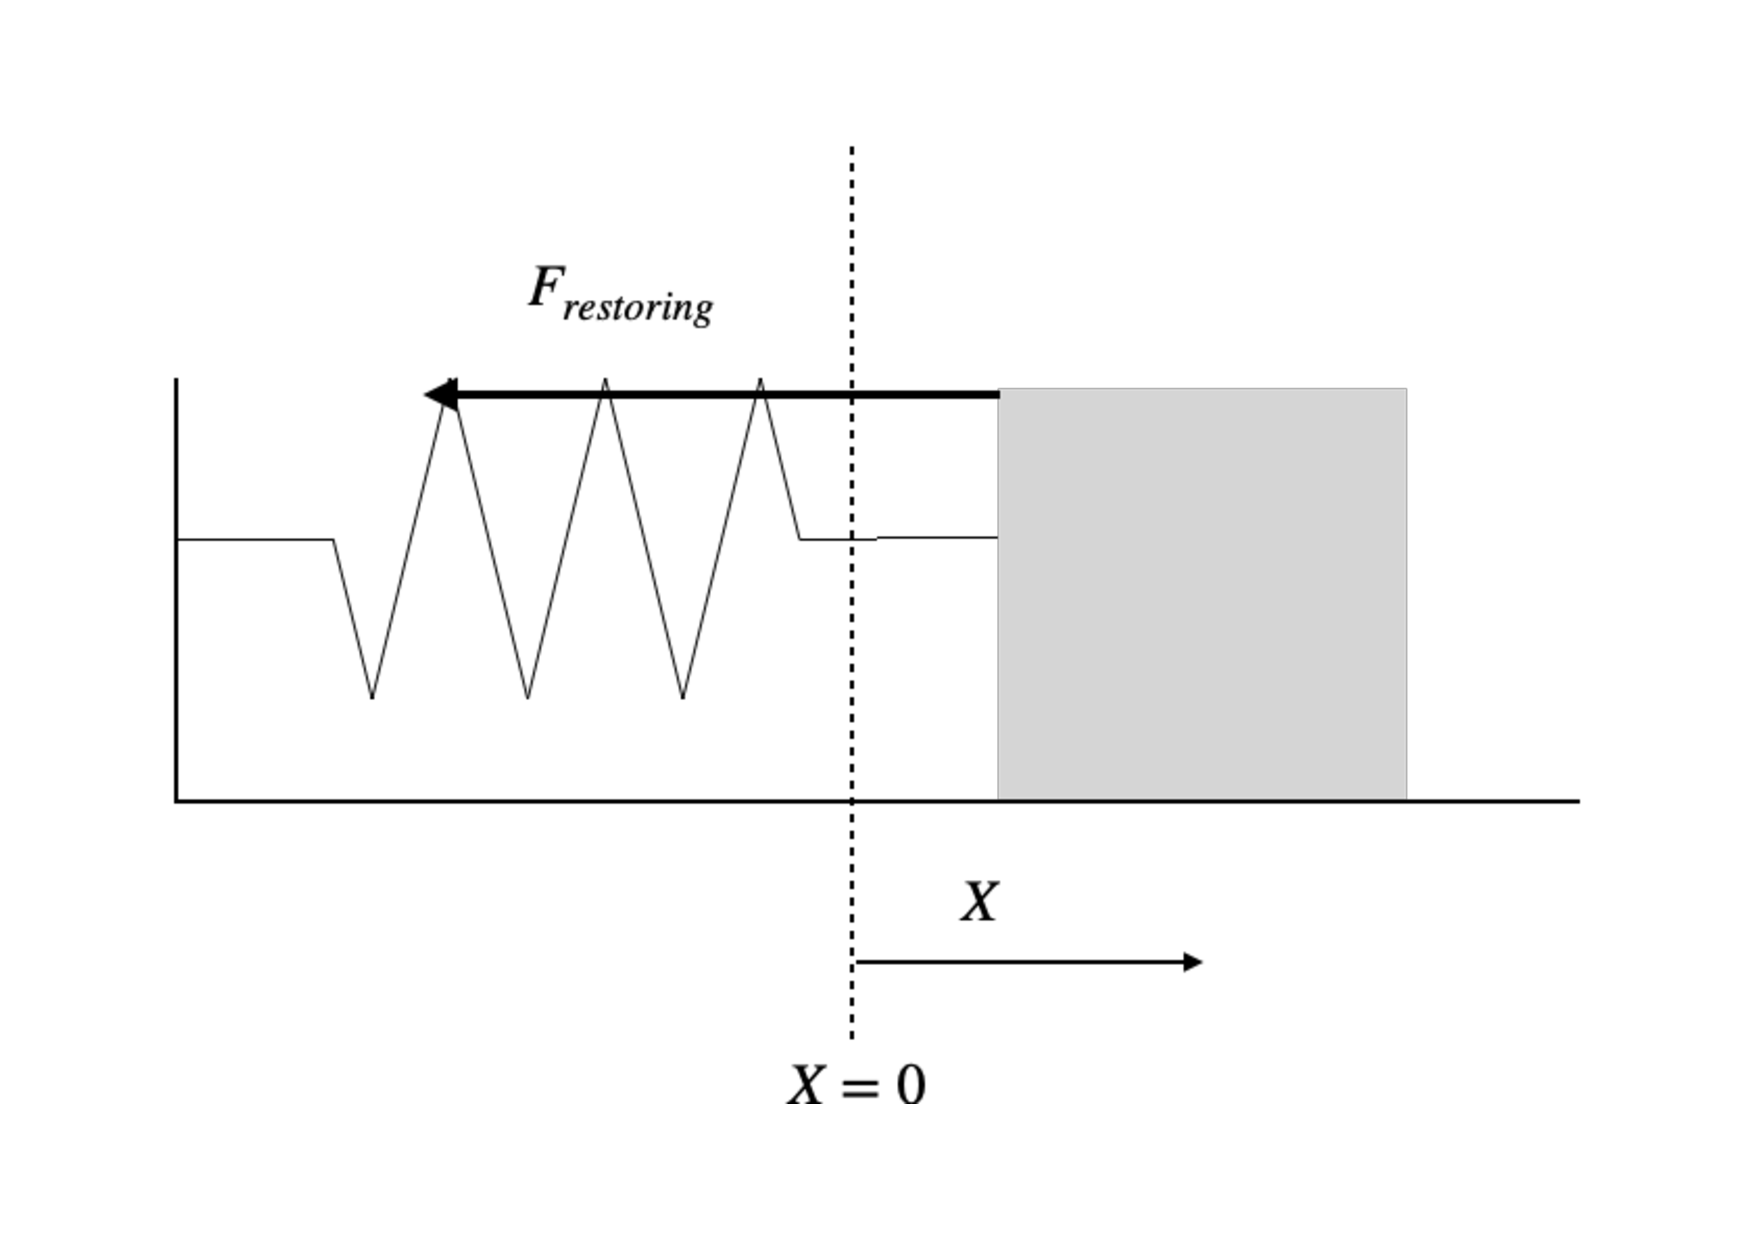
\includegraphics[trim = 50 50 50 50, width=3in]{figures/1.pdf} 
\end{center}	
The restoring force is
\[
   F_{restoring} = -kx
\]
By Newton's second law  
\[
   F_{restoring} = ma
\]
\[
-kx = ma
\]
\[
   a = -\left( \frac{k}{m}\right) x
\]

\[
   \omega = \sqrt{\frac{k}{m}},\ T = 2\pi\sqrt{\frac{k}{m}}
\]

\subsubsection{Vertical Spring mass system}
\begin{center}
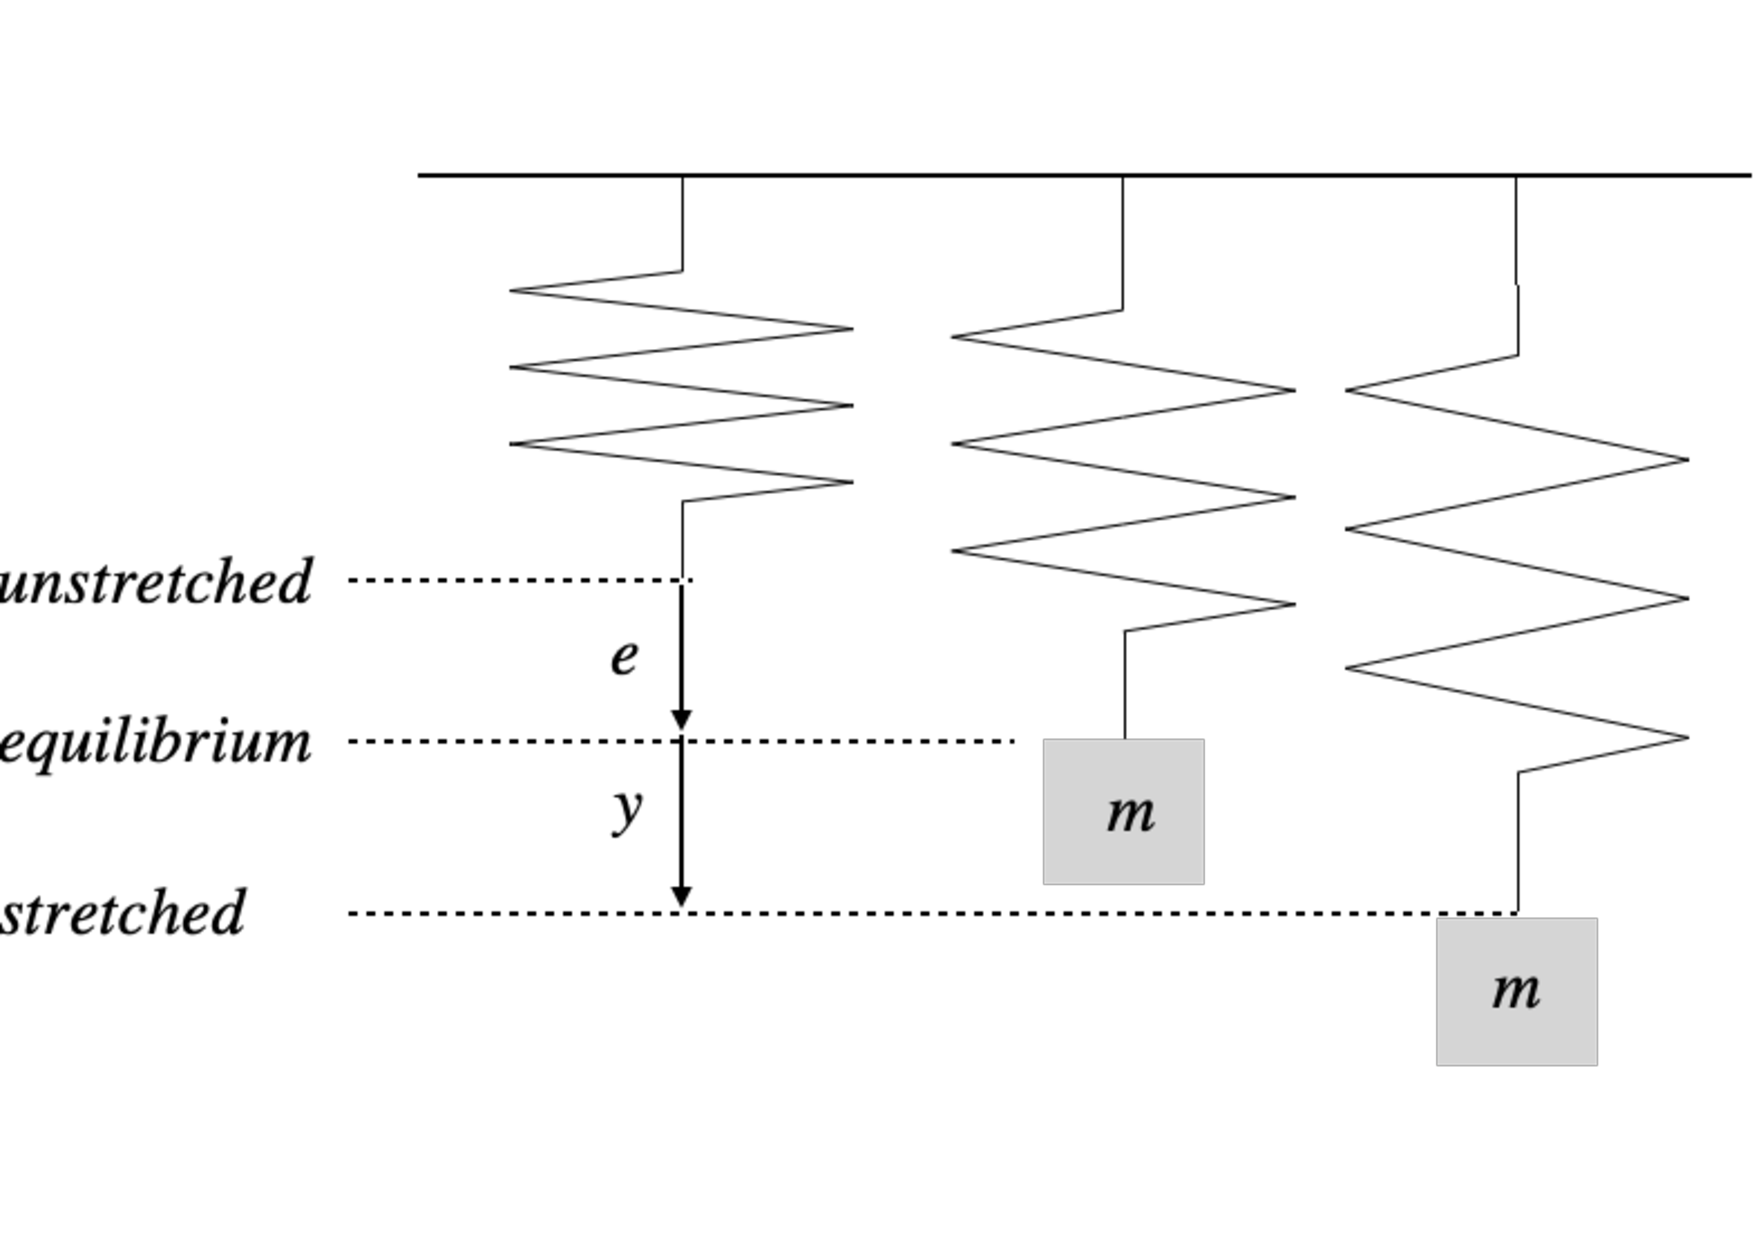
\includegraphics[trim = 50 50 50 50, width=3in]{figures/2.pdf} 
\end{center}	

The initial equilibrium is given by
\[
mg = ke
\]

when displaced by an initial $y$ 
\[
   F_{restoring} = -k(e+y) + mg
\]

by Newton's second law
\[
   F_{restoring} = mg
\]
\[
-k(e+y) + mg = ma
\]
\[
-ky = ma
\]
hence, 
\[
   a = -\left( \frac{k}{m}\right)y,\ \omega = \sqrt{\frac{k}{m}},\ T = 2\pi \sqrt{\frac{m}{k}}
\]

\subsubsection{Simple Pendulum}
\begin{center}
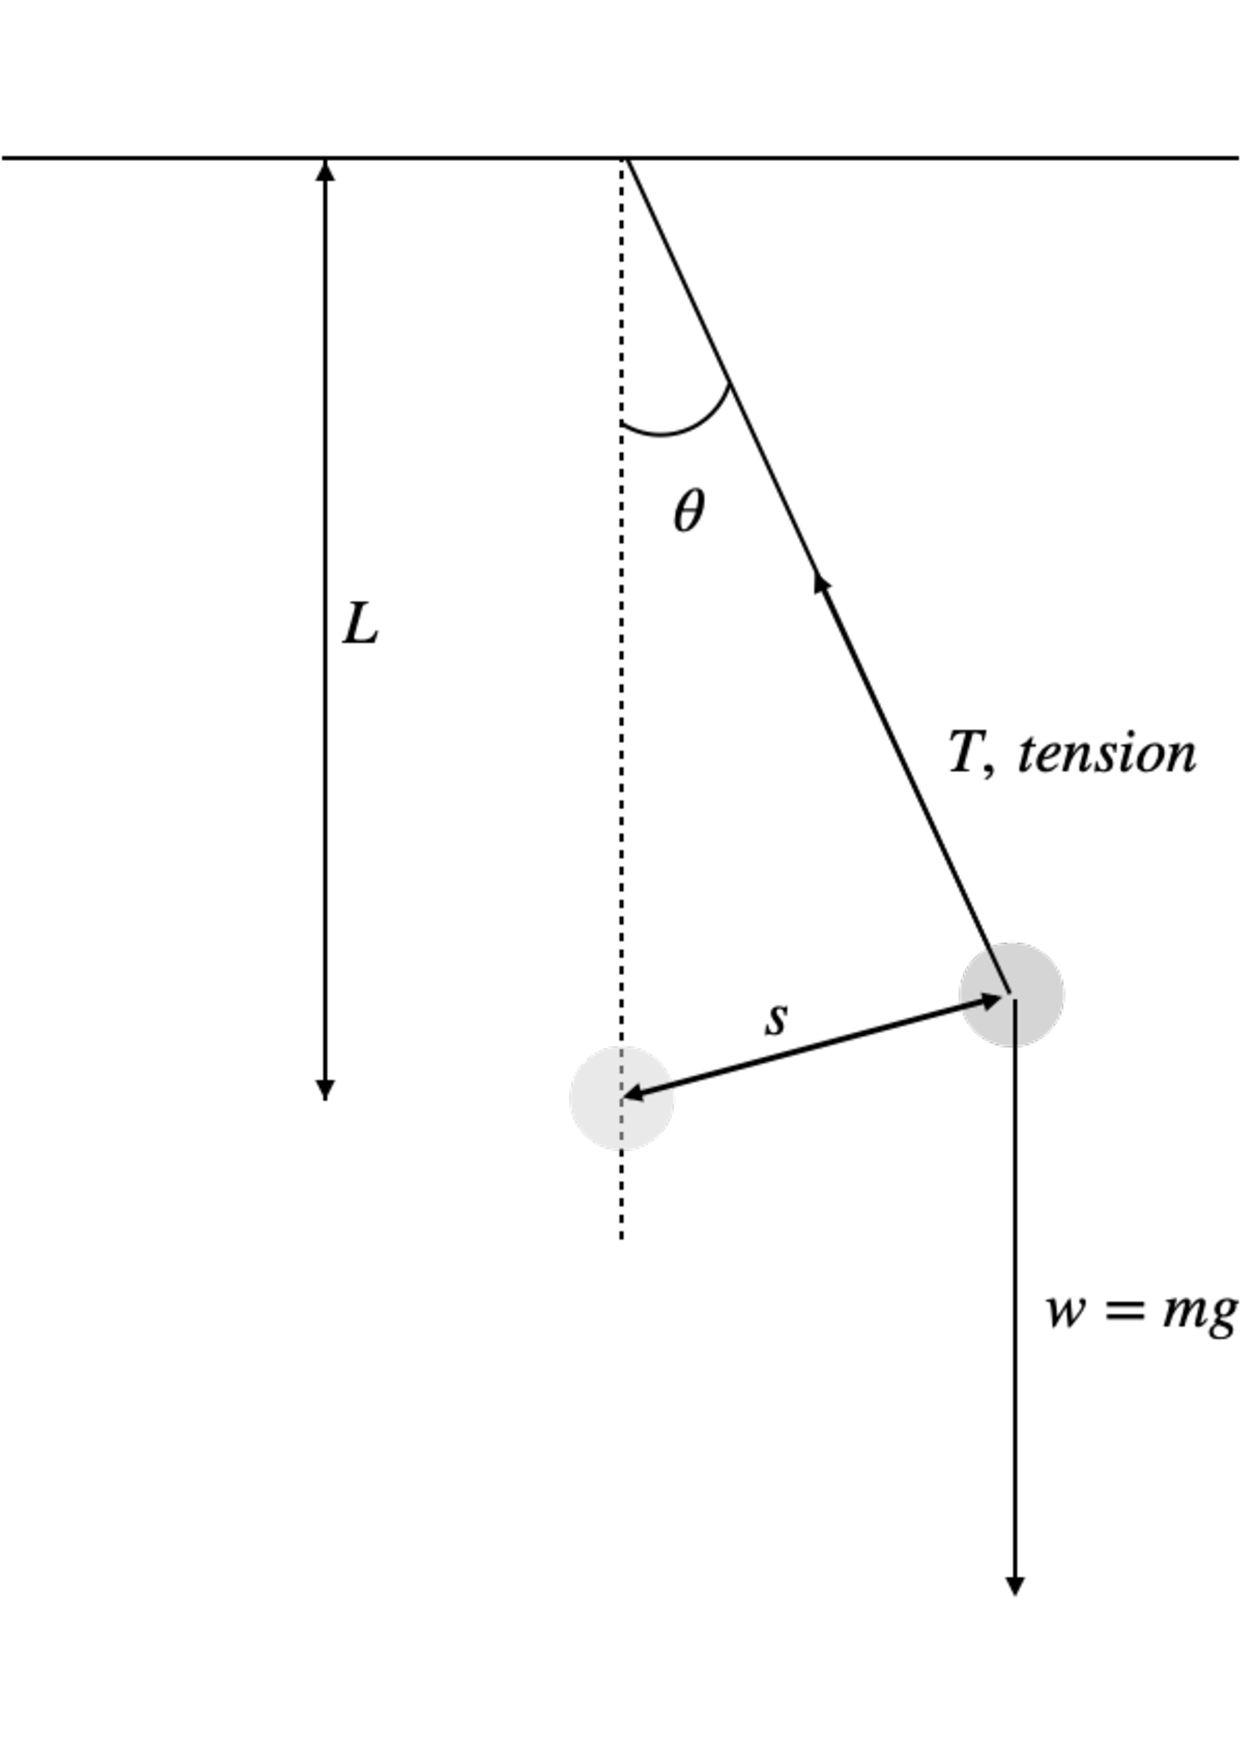
\includegraphics[trim = 50 50 50 50, width=2in]{figures/3.pdf} 
\end{center}	

\[
   F_{restoring} = -mg sin\theta
\]

For small $\theta$ $\sin \theta \cong \theta$, hence
\[
   F_{restoring} \cong -mg \theta = - mg \frac{s}{L}
\]

By Newton's Second Law
\[
   F_{restoring} = ma
\]
\[
-mg \frac{s}{L} = ma
\]
Hence, 
\[
   a = - \left( \frac{g}{L}\right)s, \ \ \omega = \sqrt{\frac{g}{L}},\ \ T = 2\pi \sqrt{\frac{L}{g}}
\]

\section{Energy in Simple Harmonic Motion}
For a horizontal spring mass system \\
KE is given by
\begin{align*}
   E_k &= \frac{1}{2} mv^2 \\
       &= \frac{1}{2} m \left( \pm \omega \sqrt{x_0^2 - x^2}\right)^2\\
       &= \frac{1}{2} m \omega^2 \left( x_0^2 - x^2\right)
\end{align*}	

PE is given by
\[
E_p = \frac{1}{2} kx^2 
\]
and since $\omega = \sqrt{\frac{k}{m}}$, 
\[
E_p = \frac{1}{2} m \omega^2 x^2
\]

Total energy is thus
\[
E = \frac{1}{2}m\omega^2 x^2
\]

\subsection{Variations of energy with time}
suppose $x = x_0 cos\omega t$, substituting $v = -x_0 \omega sin \omega t$ 
\[
   E_k = \frac{1}{2} mv^2 = \frac{1}{2} m \omega^2 x_0^2 sin^2 \omega t
\]

\[
E_p = \frac{1}{2}kx^2 = \frac{1}{2} m \omega^2 x_0^2 cos^2 \omega t
\]


\section{Damping and forced oscillations}
\subsection{Damping}
\begin{framed}
   \textbf{Damping} is the process where energy is removed from an oscillating system
\end{framed}	
\begin{itemize}
   \item \textbf{Light damping}: amplitude decays exponentially with time. Frequency decreases
   \item \textbf{Critical Damping}: results in no oscillation, and system returns to equilibrium position in the \textbf{shortest time}
   \item \textbf{Heavy Damping}: results in no oscillations and the system takes a long time to return to equilibrium position
\end{itemize}	

\subsection{Forced oscillation and resonance}
\begin{framed}
   Forced oscillations are produced when a body is subjected to a periodic external driving force
\end{framed}	

\begin{center}
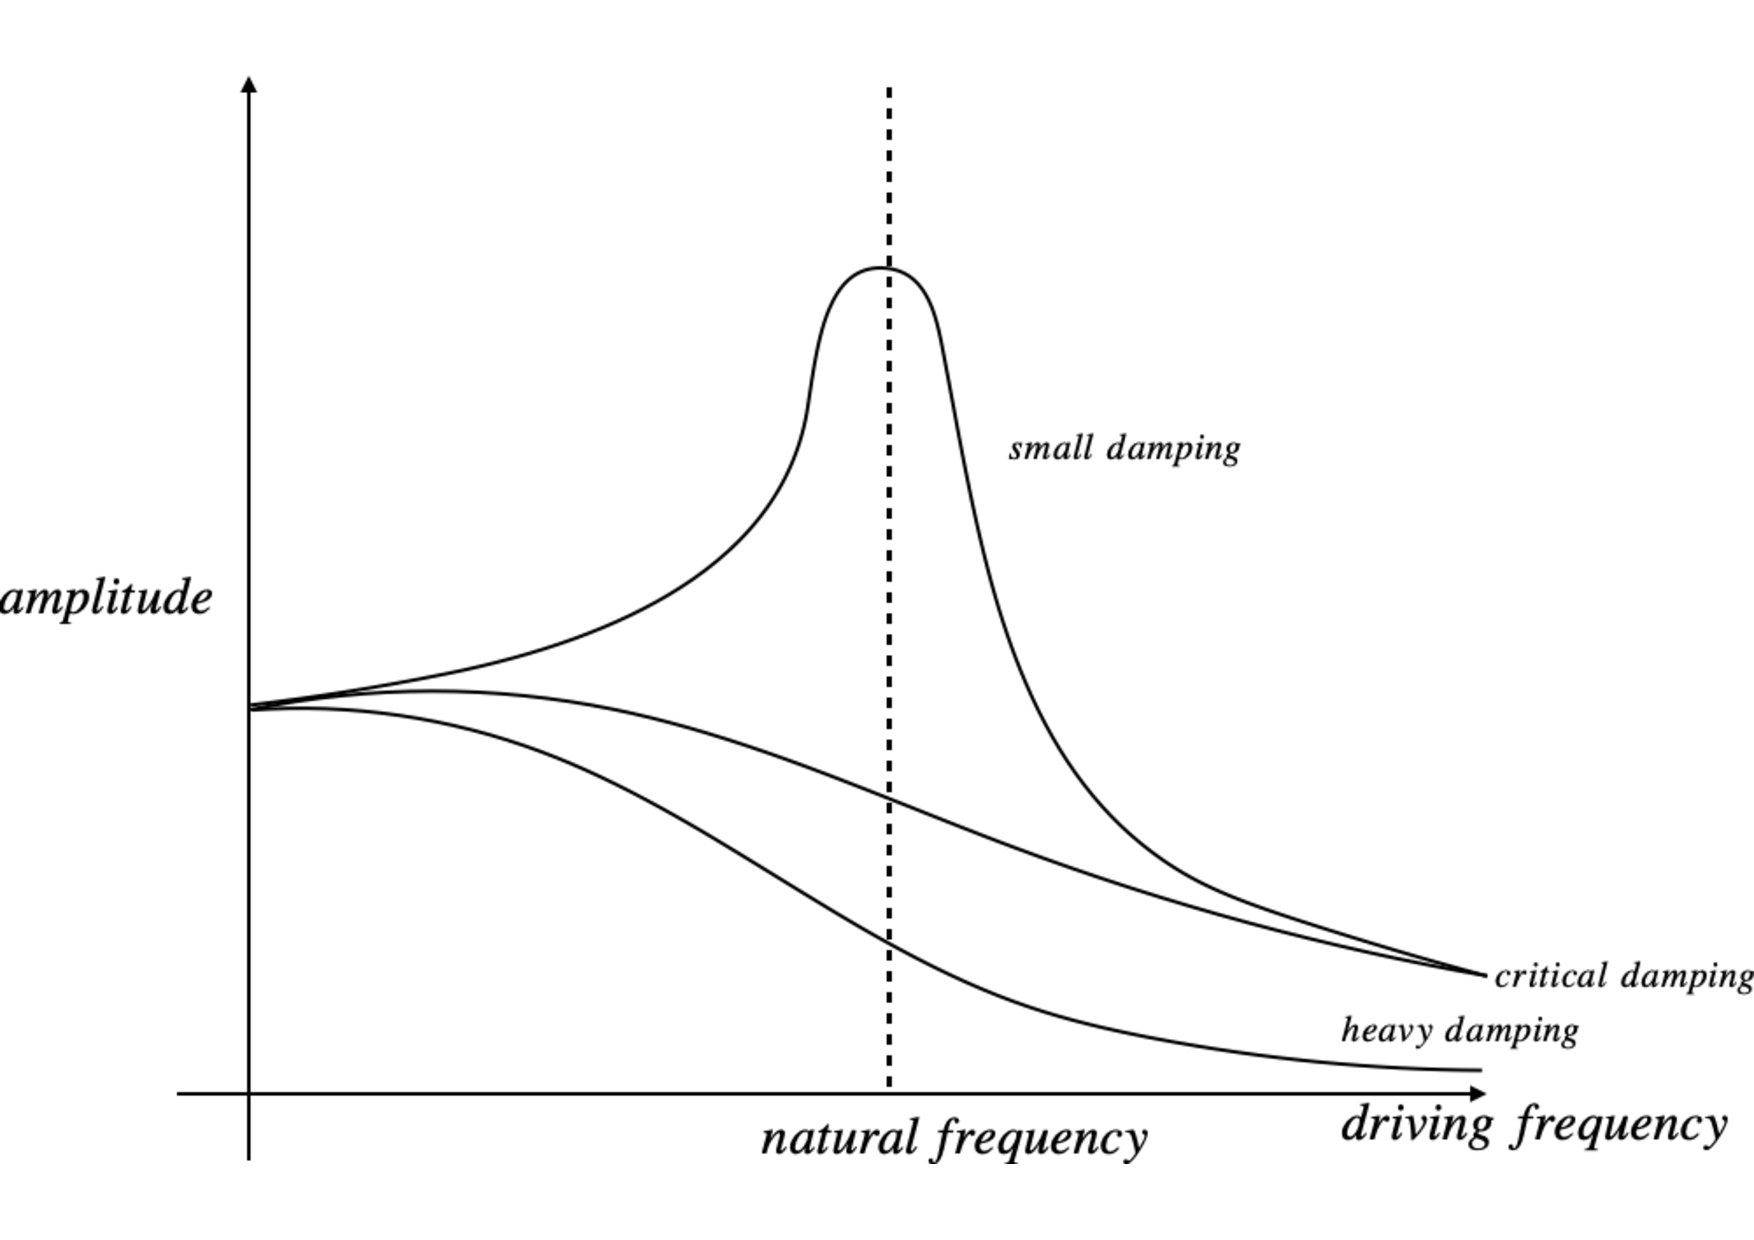
\includegraphics[trim = 50 50 50 50, width=3in]{figures/4.pdf} 
\end{center}	

\begin{framed}
   \textbf{Resonance} occurs when a system responds at maximum frequency to an external driving force. This occurs when the frequency of the driving force is equal to the natural frequency of the driving system
\end{framed}	
Circumstances where resonance is useful
\begin{itemize}
   \item Radio receiver
   \item Acoustic resonance for musical instruments
   \item Magnet resonance in MRI
\end{itemize}	

Circumstances where resonance is undesirable
\begin{itemize}
   \item Mechanical damange to structures
\end{itemize}	

\end{document}	





